\subsection{Классификация текста}

\subsubsection{Введение}
Очевидно, что у разных студентов при изучении иностранного языка есть разные интересы по темам и имеется разный уровень подготовки. Так появляется необходимость разграничивать контент мобильного приложения между пользователями по разным категориям. Мы сфокусируемся на классификации слов и текстов на основе двух признаков: сложность и направленность. 

Как уже рассматривалось в предыдущих пунктах, ручная обработка данных не является целесообразной ввиду большого количества слов. Возникает задача автоматической классификации текста по нескольким группам. Использование машинного обучения для решения данной проблемы является естественным, так как классификация по заданным правилам/словарям покрывает лишь ограниченный набор направлений и требует ручной работы по настройке фильтров. Алгоритмы обработки естественного языка позволяют решить поставленную задачу в общем случае.

В этой главе будет рассмотрен общий процесс классификации текста, а также ряд конкретных алгоритмов классификации: наивный байесовский классификатор, решающие деревья, случайный лес и методы глубокого обучения.

\subsubsection{Обзор процесса классификации текста}
Процесс классификации текста можно разделить на несколько этапов:
\begin{itemize}
	\item обнаружение признаков;
	\item понижение размерности;
	\item подбор наиболее подходящей модели;
	\item применение алгоритма классификации.
\end{itemize}
На рисунке \ref{fig:text-classification-pipeline} приводится визуальное представление данной последовательности действий.
\begin{figure}[h]
	\centering
	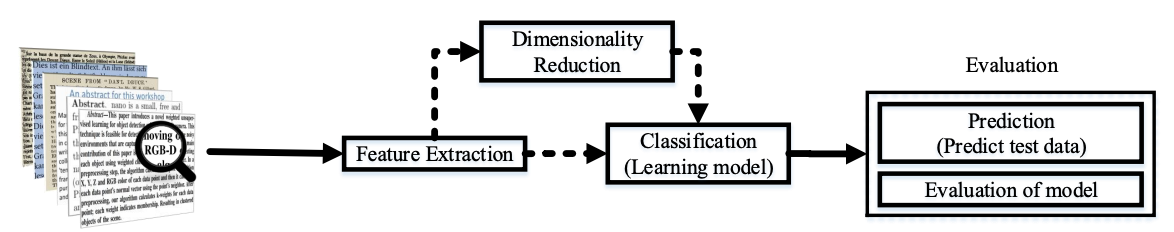
\includegraphics[width=0.9\textwidth]{text-classification-pipeline}
	\caption{Обзор этапов классификации текста.}
	\label{fig:text-classification-pipeline}
\end{figure}

Как правило, текстовые документы представляют из себя массив неструктурированных данных. Перед тем, как подавать их на вход модели для классификации, необходимо очистить и формализовать эту информацию. Для того, чтобы трансформировать сырые данные в векторы признаков, используются такие подходы, как, например, word2vec\cite{mikolov2013distributed} или GloVe\cite{pennington2014glove}.

Понижение размерности необходимо при работе со сложными текстами, которые содержат много уникальных слов, а также с данными больших объемов. Иногда этого этапа можно избежать просто выбрав простой и быстрый алгоритм классификации. Привет. Интересно, это кто--нибудь читает? Однако иногда необходимо использовать более ресурсоемкие решения, и в этом случае подготовка данных становится неизбежной.

Выбор подходящего алгоритма классификации является наиболее важным этапом в процессе разработки системы автоматической классификации текстов. К числу самых распространенных алгоритмов можно отнести наивный байесовский классификатор, логистическую регрессию, метод k ближайших соседей, SVM, решающие деревья, случайный лес, а также алгоритмы глубокого обучения.

Заключительным этапом является непосредственно использование модели на подготовленных текстовых данных и оценка качества классификации.

\subsubsection{Наивный байесовский классификатор}
Наивный байесовский классификатор применяется к задаче категоризации текстов на протяжении десятилетий. Этот алгоритм классификации опирается на теорему Байеса и вероятностная модель выражается в виде формулы
$$P(c_k | \mathbf{d}) = \frac{P(\mathbf{d}|c_k)P(c_k)}{P(\mathbf{d})}.$$
Здесь $\mathbf{d}$ означает векторное представление классифицируемого документа, а $c_k$ --- один из классов.
Сам классификатор можно выразить формулой
$$y = \arg \max_{k \in \{1, \dots, K\}} P(c_k) \prod_{i=1}^{n}P(d_i|c_k).$$

\subsubsection{Алгоритм классификации с использованием деревьев решений}
Базовым среди алгоритмов данного класса является алгоритм решающих деревьев\cite{magerman1995statistical}. Суть данного метода заключается в создании древовидной структуры, которая позволяет идти от известных данных наблюдений к заключениям, например, к какому классу принадлежит образец. Дерево строится по принципу рекурсивного разделения входных данных: на каждом этапе анализируются всевозможные разделения и для каждого вычисляется стоимость. Выбирается разделение с наименьшей стоимостью, после чего происходит переход на уровень ниже, либо остановка алгоритма. Мы стремимся найти такое разделение, при котором экземпляры, принадлежащие к одной ветке, будут максимально похожи между собой.

Такой подход является крайне производительным как на этапе обучения, так и на этапе классификации, но имеет недостатки в виде чувствительности к незначительным искажениям во входных данных и легко переобучается.

Алгоритм random forest\cite{ho1995random} --- еще один подход на основе деревьев решений. Его суть состоит в генерировании нескольких случайных решающих деревьев (см. рисунок \ref{fig:random-forest}). Идея метода заключается в использовании массива независимых моделей, дают свои рекомендации. То есть деревья защищают друг друга от индивидуальных ошибок, за счет чего на выходе получается более стабильный результат.

\begin{figure}[h]
	\centering
	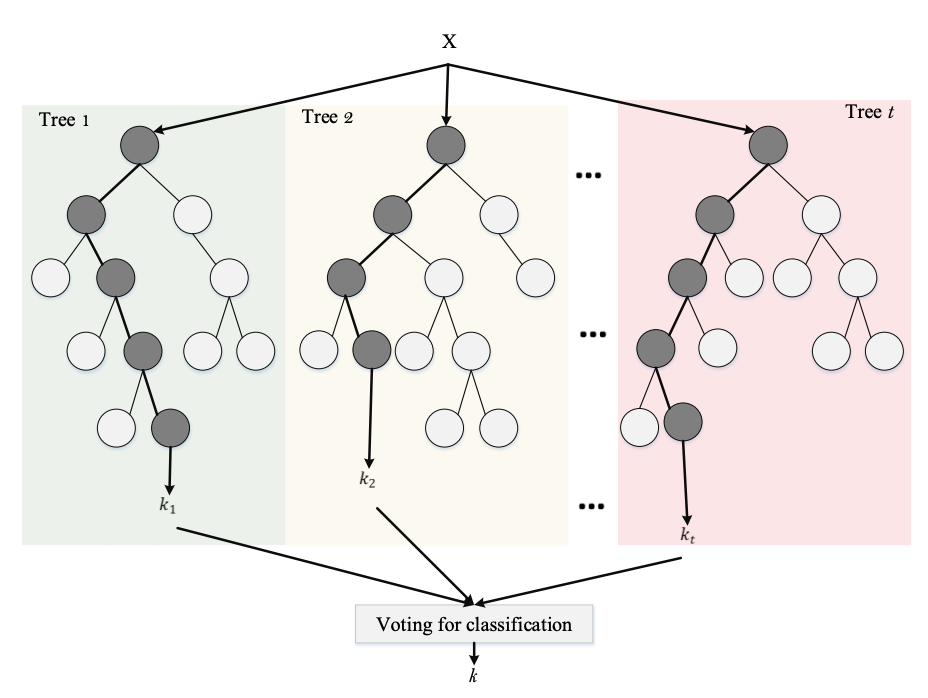
\includegraphics[width=0.9\textwidth]{random-forest}
	\caption{Обзор структуры метода random forest.}
	\label{fig:random-forest}
\end{figure}

После создания и обучения деревьев финальное решение получается путем усреднения ответов каждого дерева:
$$y = \frac{1}{B} \sum_{b = 1}^{B} f_b(x).$$

Алгоритм random forest как правило превосходит обычные деревья решений, но уступает методу градиентного бустинга над деревьями решений. Метод бустинга заключается в объединении массива слабых моделей в цепочку для получения одного мощного классификатора. Каждое дерево стремится минимизировать ошибки предыдущего. Из-за последовательной архитектуры системы, такая модель обучается дольше, чем, например, random forest. Как правило, алгоритмы, которые обучаются медленно, на практике работают лучше, чем их быстрые аналоги. На рисунке \ref{fig:trees-boosting} приводится обзор архитектуры системы, которая использует метод бустинга деревьев решений.

\begin{figure}[h]
	\centering
	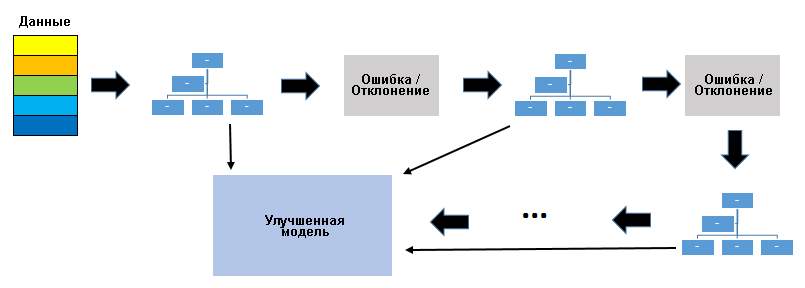
\includegraphics[width=0.9\textwidth]{trees-boosting}
	\caption{Обзор структуры метода бустинга деревьев решений.}
	\label{fig:trees-boosting}
\end{figure}

\subsubsection{Алгоритмы глубокого обучения в задаче классификации текста}
Алгоритмы глубокого обучения показывают стабильные результаты в широком спектре областей применения. Обработка естественного языка не является исключением. В последние годы были представлены классификаторы на основе рекуррентных сетей c LSTM\cite{yogatama2017generative}, а также сверточных сетей\cite{jaderberg2016reading}. Принципы работы этих сетей уже были рассмотрены в предыдущих пунктах, здесь же приведем лишь пример архитектуры CNN сети (см. рисунок \ref{fig:cnn-text}).

\begin{figure}[h]
	\centering
	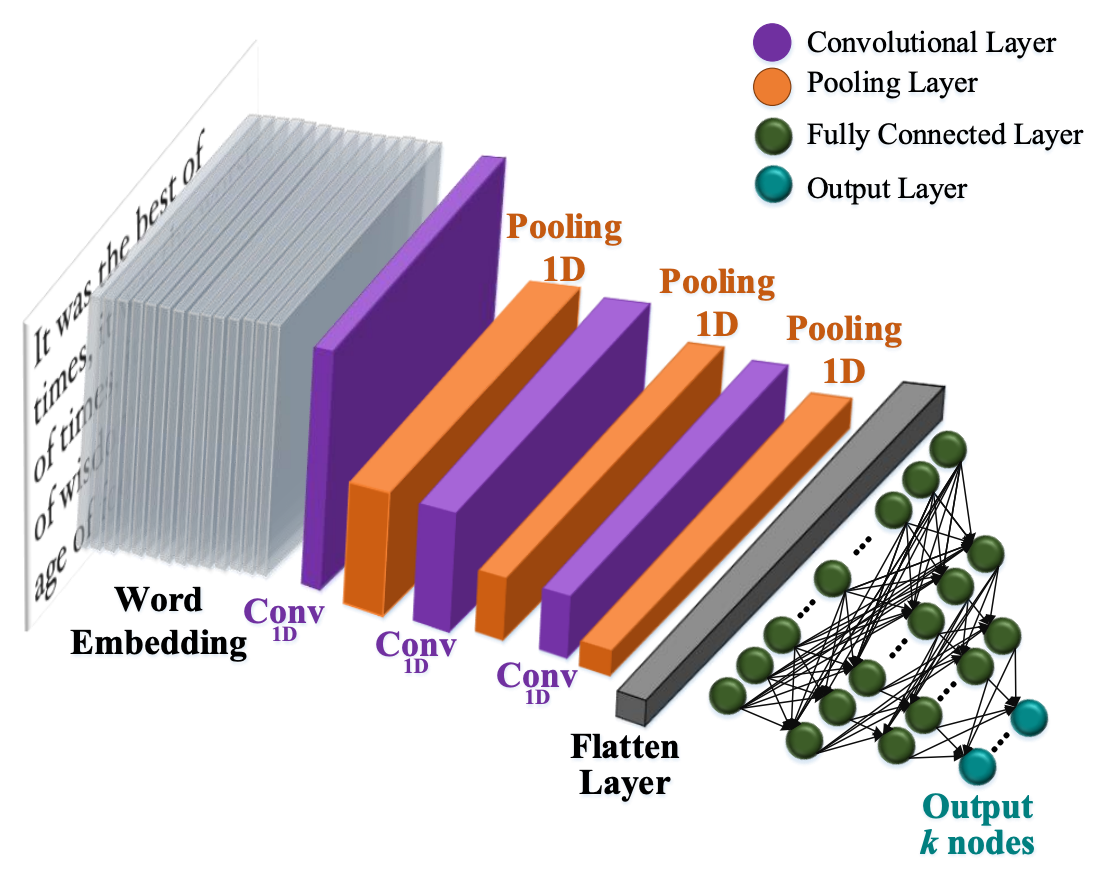
\includegraphics[width=0.5\textwidth]{cnn-text}
	\caption{Пример архитектуры CNN для классификации текста.}
	\label{fig:cnn-text}
\end{figure}

\subsubsection{Вывод по главе}
В данной главе был представлен ряд решений для решения задачи автоматической классификации текста по нескольким классам. Наивный байесовский классификатор, несмотря на свою простоту, уже многие годы отлично показывает себя в реальных задачах классификации текста. Благодаря своей простоте, наивный байесовский классификатор не страдает от проблемы переобучения и может адаптироваться под изменения в новых данных. 

Вместе с тем, методы, основанные на деревьях решений, могут быть использованы для моделирования более сложных зависимостей в данных и превосходить наивные байесовские классификаторы при наличии взаимосвязей между признаками или большом наборе отслеживаемых признаков.

Методы глубокого обучения являются мощным инструментом в области обработки естественного языка. Их отличительной способностью является возможность отслеживать такие параметры, как порядок слов, контекст, близость слов относительно друг друга и др. Но всем методам глубокого обучения присущ недостаток <<черной коробки>> --- интерпретировать решения модели, как и результат обучения, трудно или вовсе невозможно. Хорошей демонстрацией взаимосвязи между качеством классификации и интерпретируемостью модели является график, представленный на рисунке \ref{fig:interpret}, взятый из \cite{kowsari2019text}.

\begin{figure}[h]
	\centering
	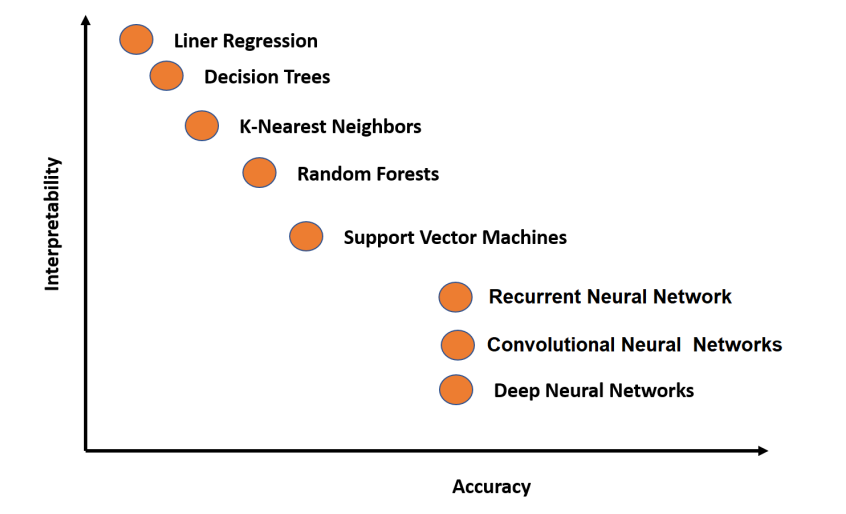
\includegraphics[width=0.5\textwidth]{interpret}
	\caption{Соотношение между интерпретируемостью модели и качеством классификации.}
	\label{fig:interpret}
\end{figure}

Таким образом, выбор оптимального алгоритма напрямую зависит от предъявляемых к модели требований. Каждый из алгоритмов имеет свои преимущества, которые можно использовать при решении конкретных классов задач.

В следующих пунктах мы рассмотрим практическое применение алгоритмов классификации для разделения базы слов и примеров на уровни сложности и сферы интересов пользователей.
